% Figure 1 composite assembly (vector-preserving) for AllelePerturb.
% 7 panels: a task-def, b tracks+legend, c depth, d features+PCA, e evaluation,
% f splits, g workflow. Build: pdflatex fig1_assemble.tex -> fig1_assemble.pdf
\documentclass[tikz,border=1mm]{standalone}
\usepackage{graphicx}
\usepackage{helvet}
\renewcommand{\familydefault}{\sfdefault}
\begin{document}
\begin{tikzpicture}[x=1mm,y=1mm]
  % crop to content (bottom margin removed)
  \useasboundingbox (0,32) rectangle (183,203);

  % ---------- Row 1: a (task definition) | b (variant tracks + legend) ----------
  \node[anchor=north west,inner sep=0] at (5,198) {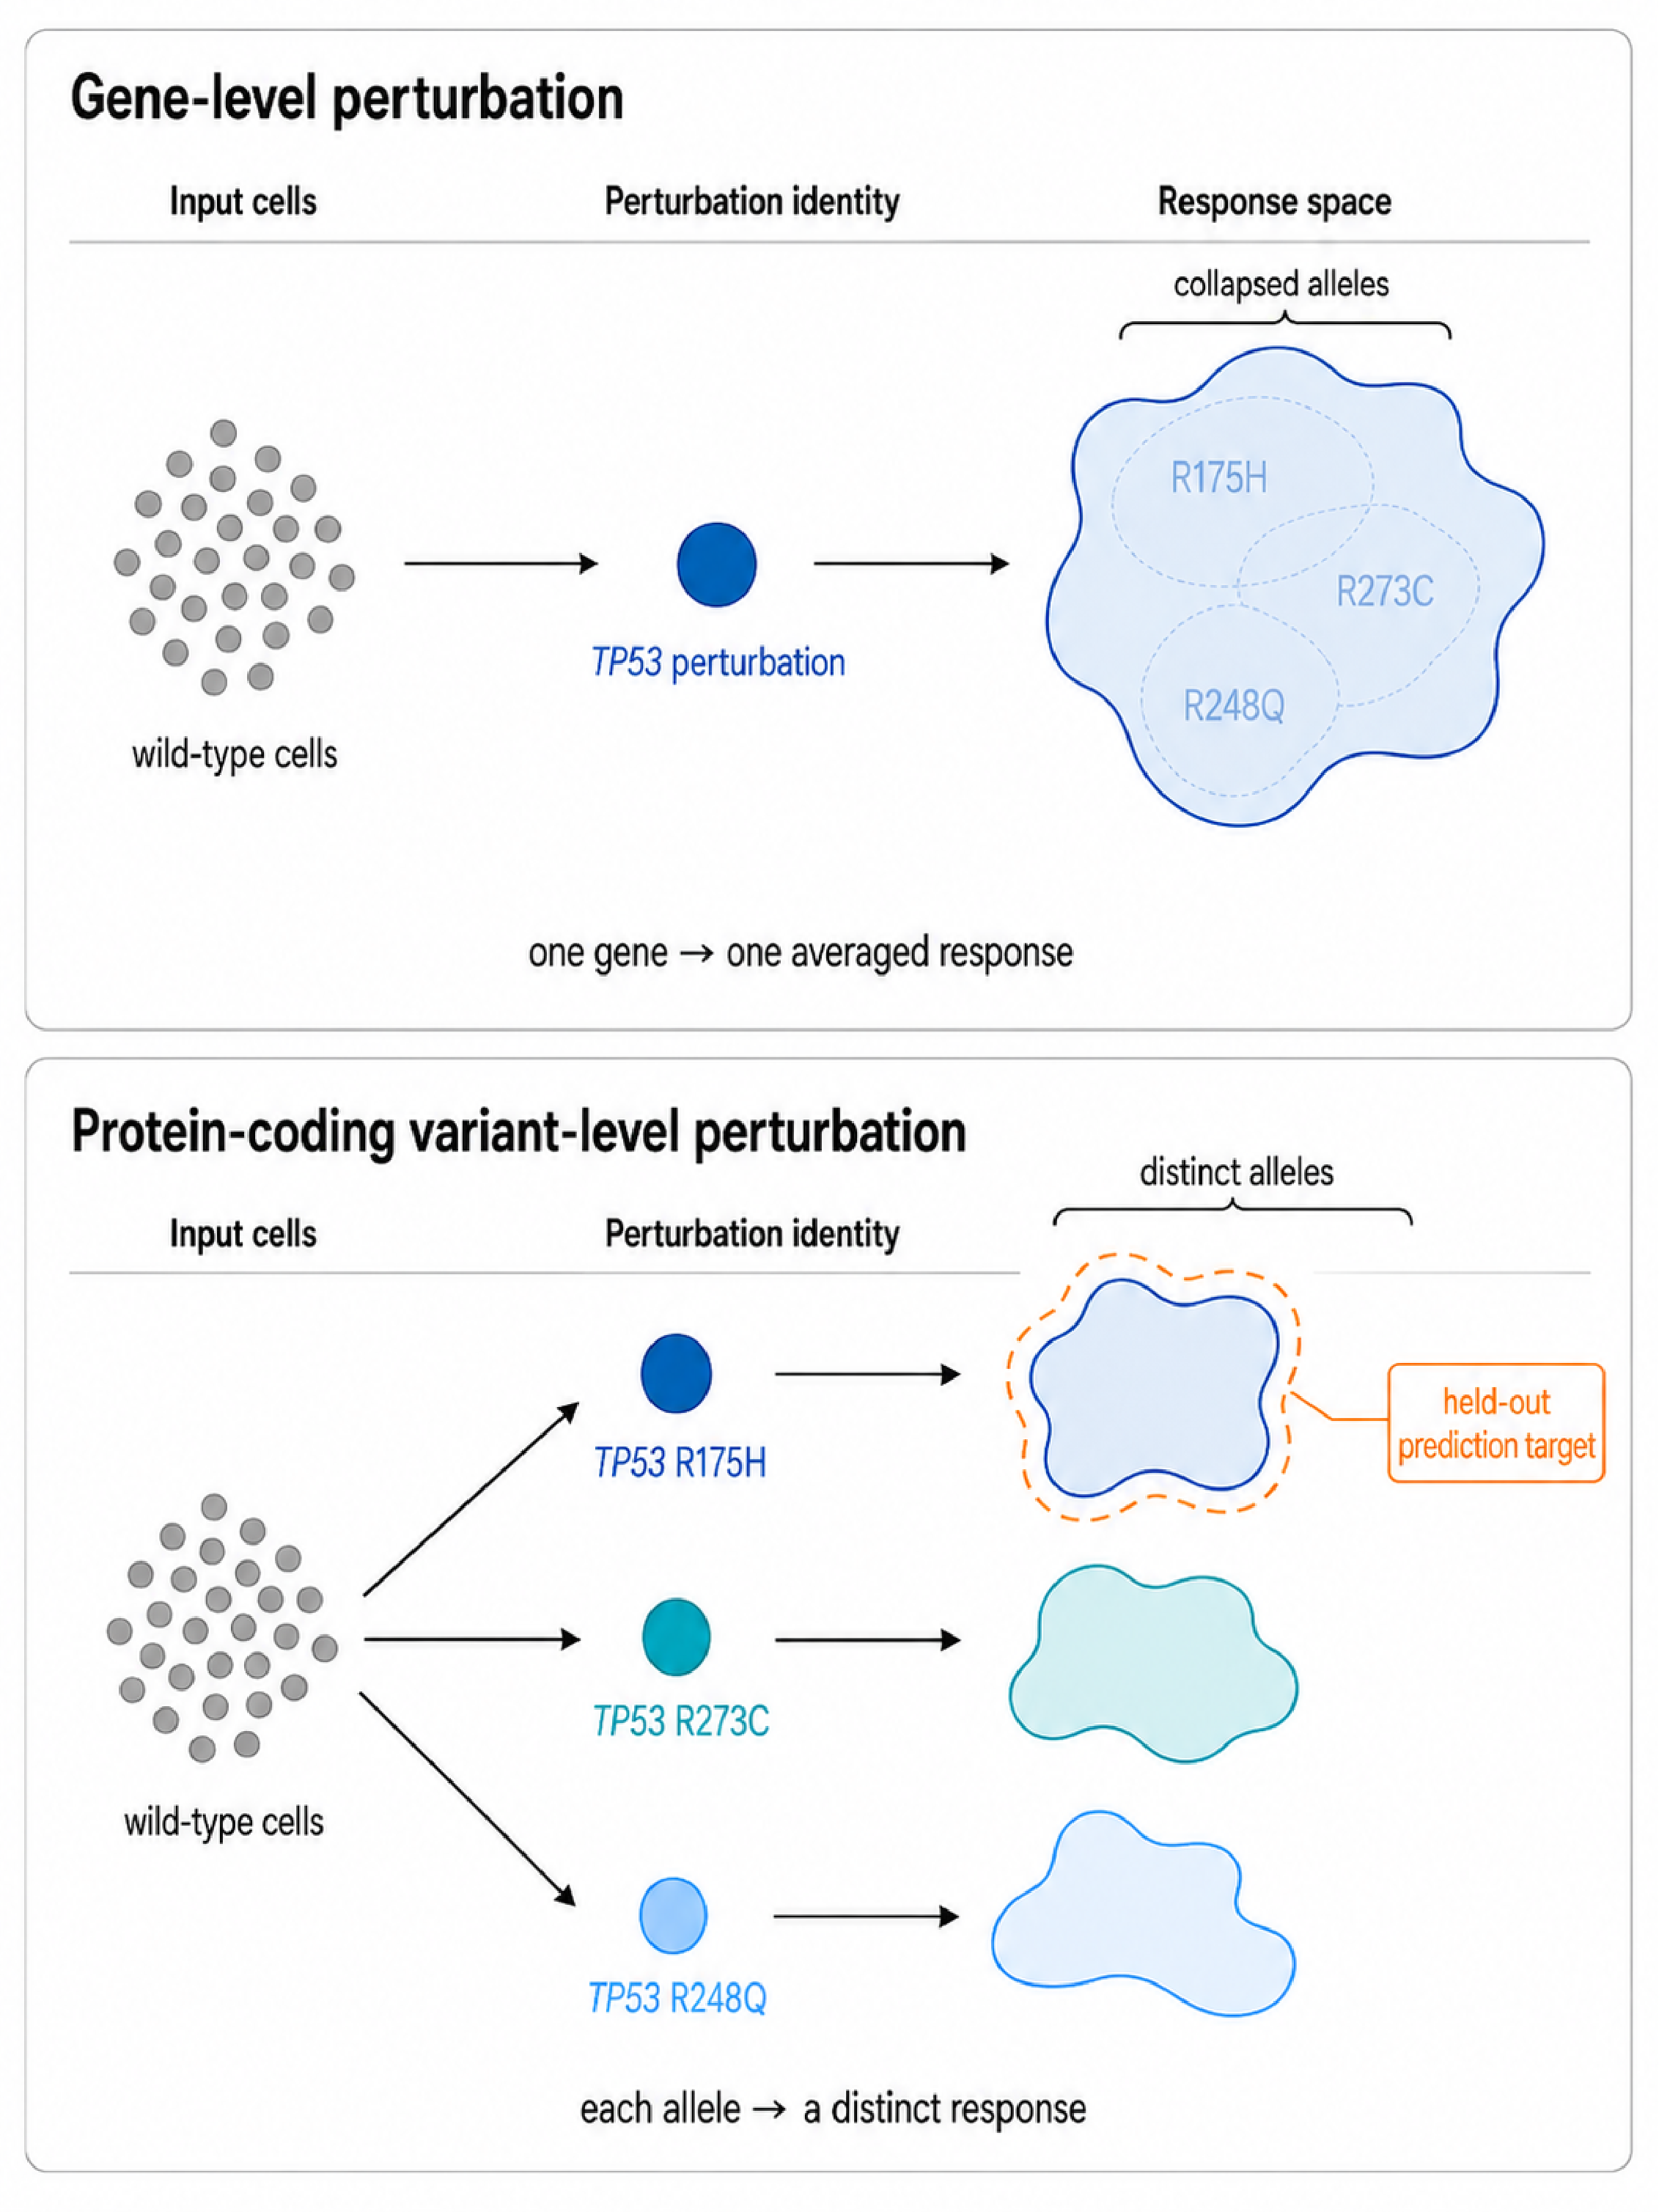
\includegraphics[width=60mm]{Fig1a.pdf}};
  \node[anchor=north west,inner sep=0] at (72,199)
    {\begin{minipage}{57mm}
       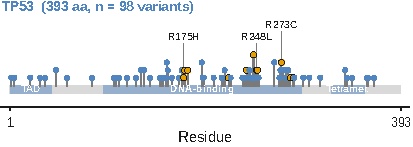
\includegraphics[width=\linewidth]{fig1b_track_TP53.pdf}\\[-0.3mm]
       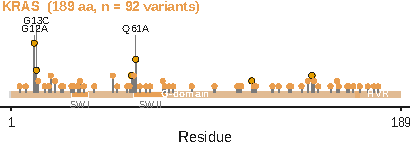
\includegraphics[width=\linewidth]{fig1b_track_KRAS.pdf}\\[-0.3mm]
       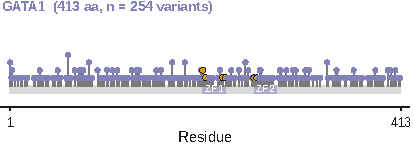
\includegraphics[width=\linewidth]{fig1b_track_GATA1.pdf}\\[-0.3mm]
       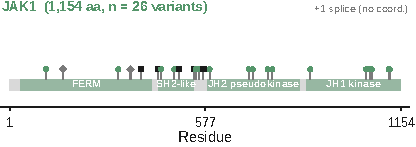
\includegraphics[width=\linewidth]{fig1b_track_JAK1.pdf}\\[0.4mm]
       \hspace*{7mm}
\includegraphics[width=35mm]{fig1b_legend.pdf}
     \end{minipage}};

  % ---------- Row 2: c (depth) | d (features + PCA inset) | e (evaluation) ------
  % equal ~37 mm heights so the row bottom is flush
  \node[anchor=north west,inner sep=0] at (5,110)  {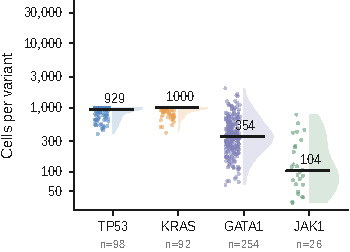
\includegraphics[width=52mm]{fig1c_depth.pdf}};
  \node[anchor=north west,inner sep=0] at (60,110) {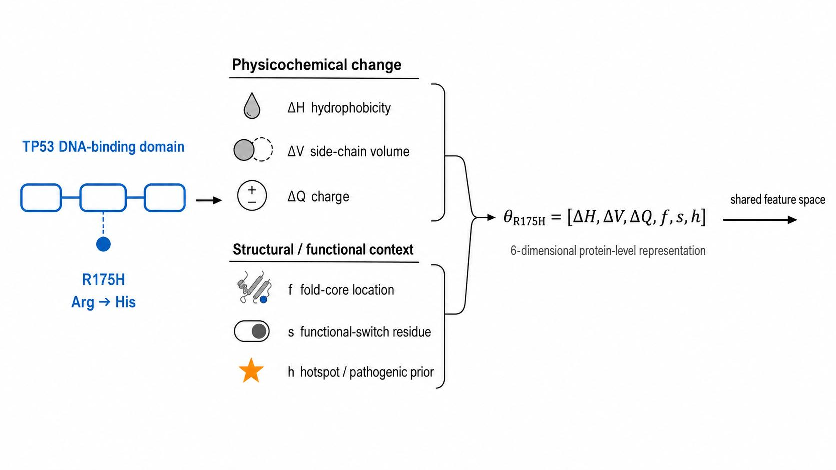
\includegraphics[width=66mm]{Fig1d_schematic_highres.pdf}};
  \node[anchor=north west,inner sep=0] at (101,103){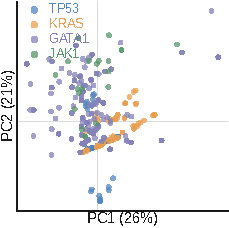
\includegraphics[width=22mm]{fig1d_theta_pca.pdf}};
  \node[anchor=north west,inner sep=0] at (129,110){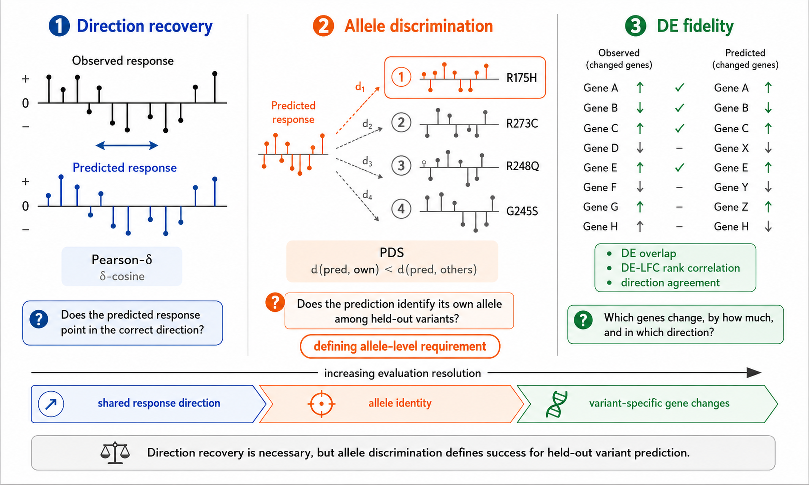
\includegraphics[width=52mm]{Fig1e_Eval_highres.pdf}};

  % ---------- Row 3: f (splits) | g (workflow) ---------------------------------
  \node[anchor=north west,inner sep=0] at (5,68)  {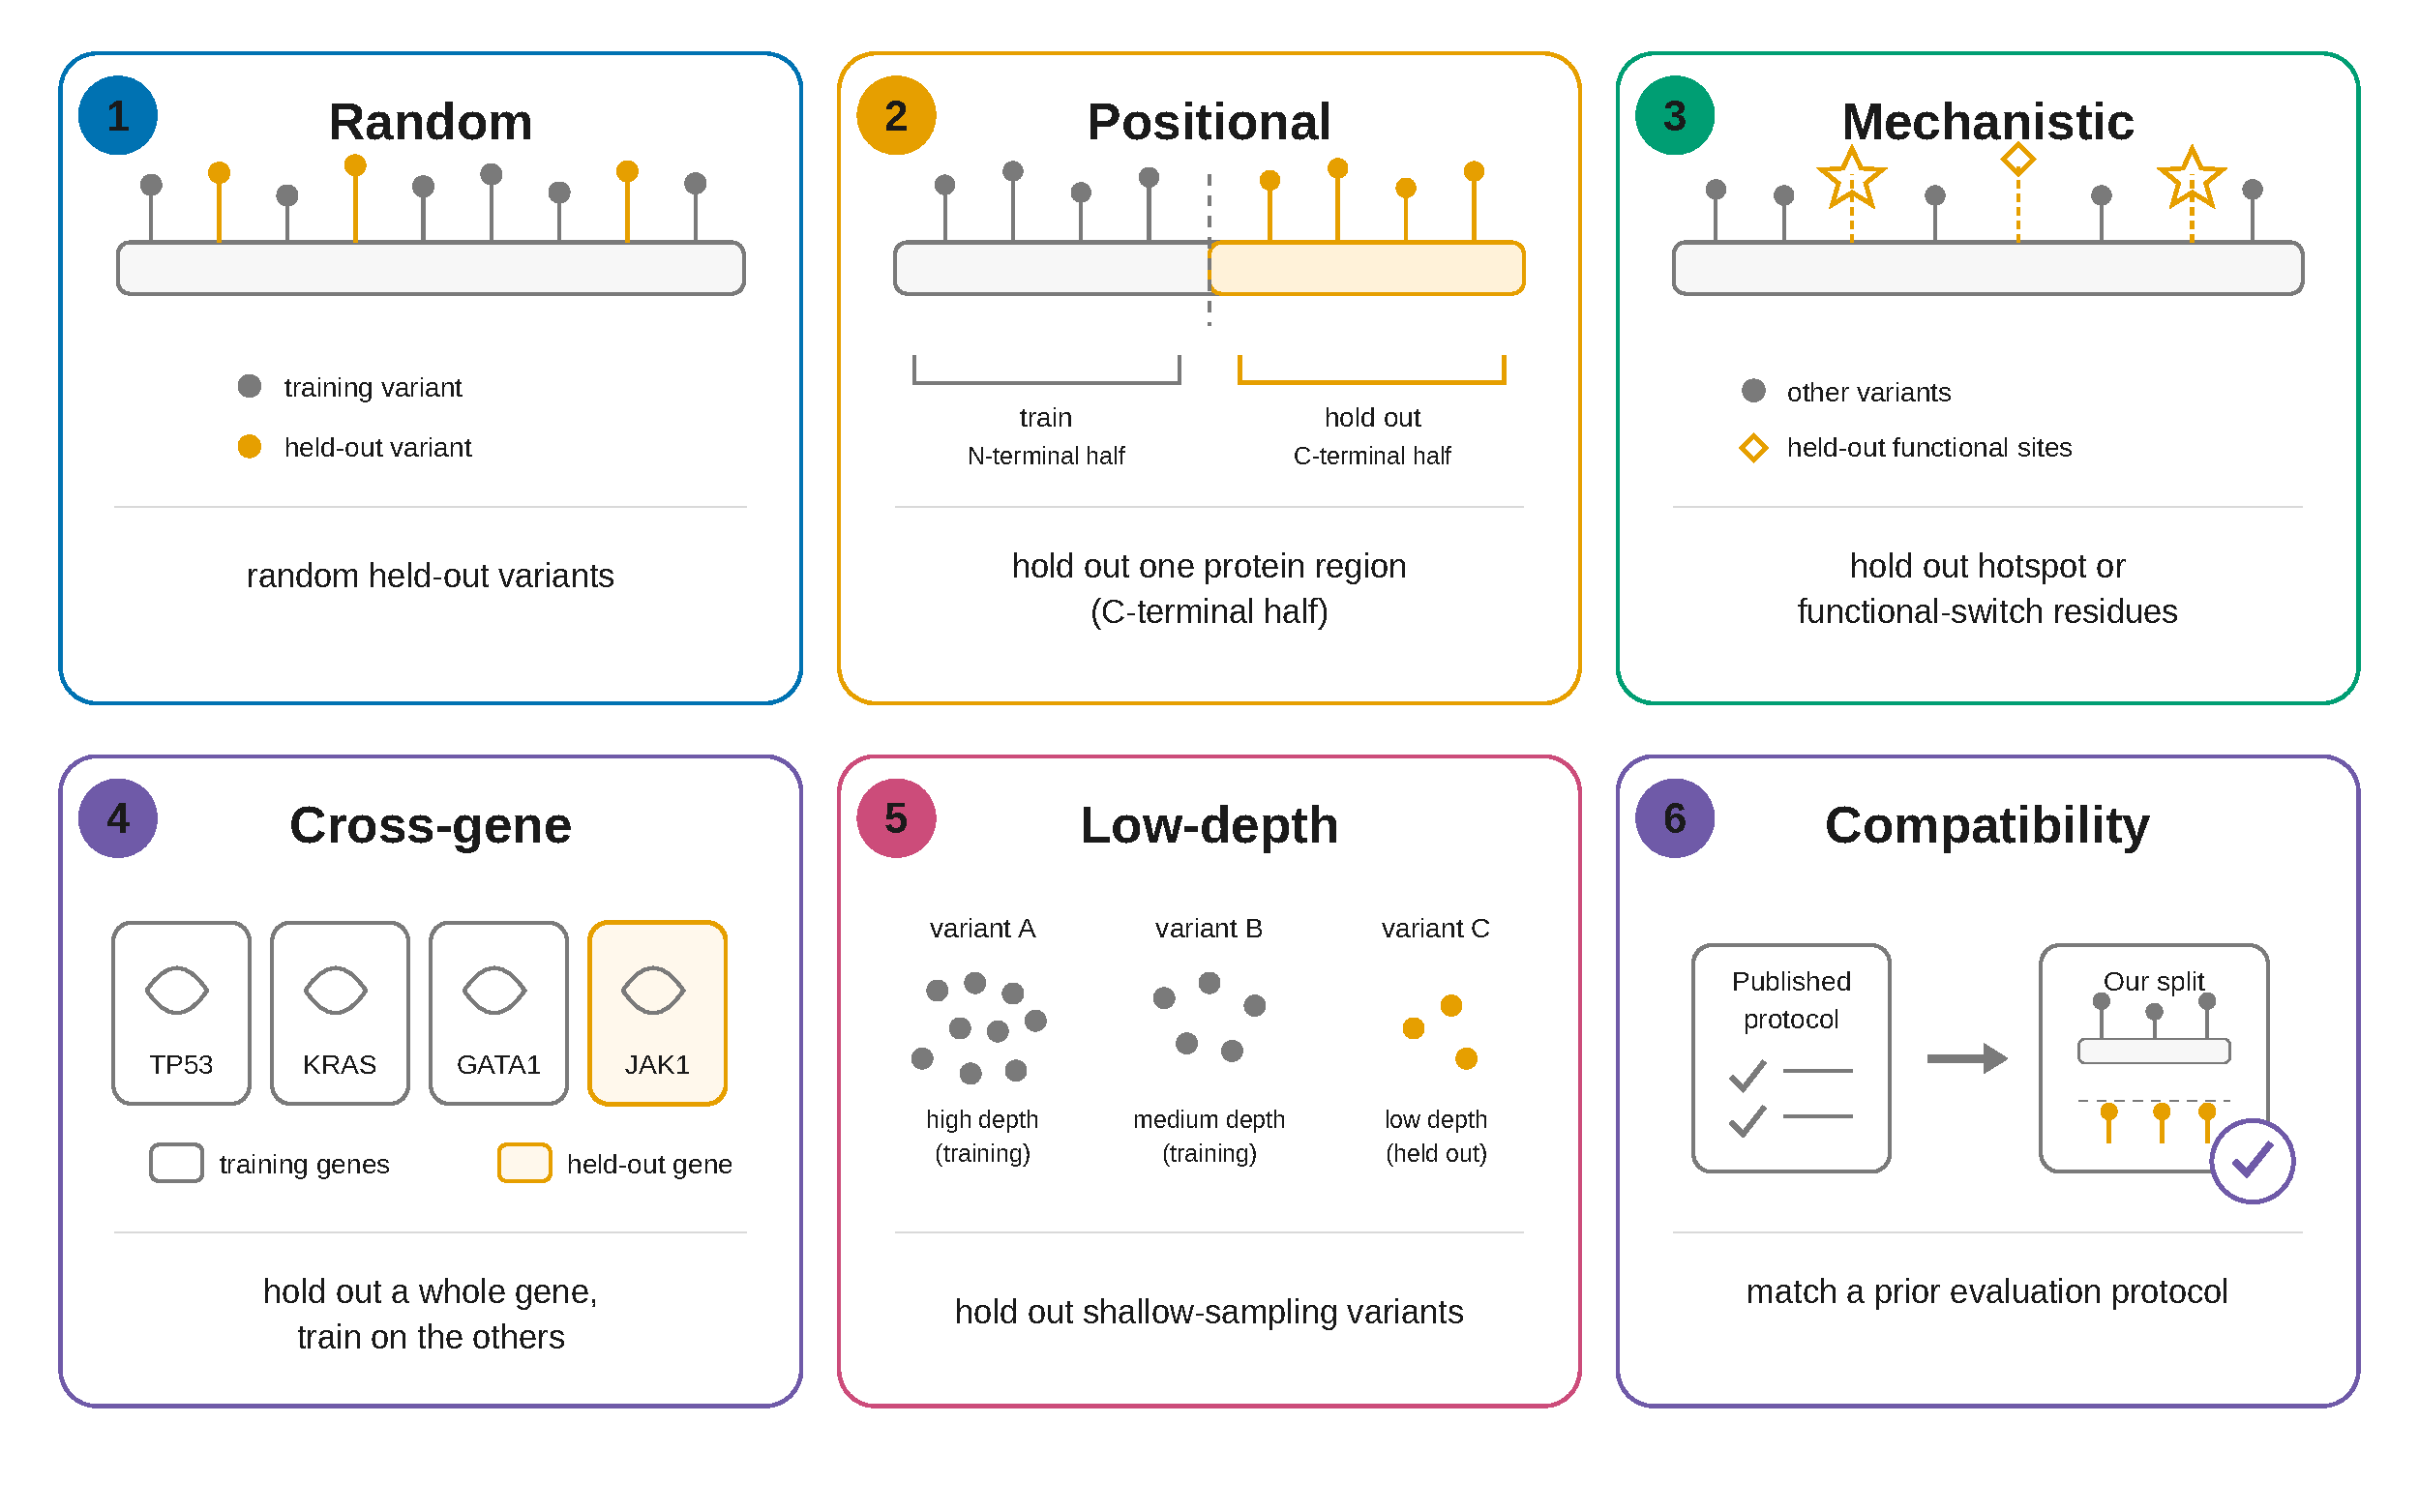
\includegraphics[width=60mm]{Fig1f.pdf}};
  \node[anchor=north west,inner sep=0] at (69,64) {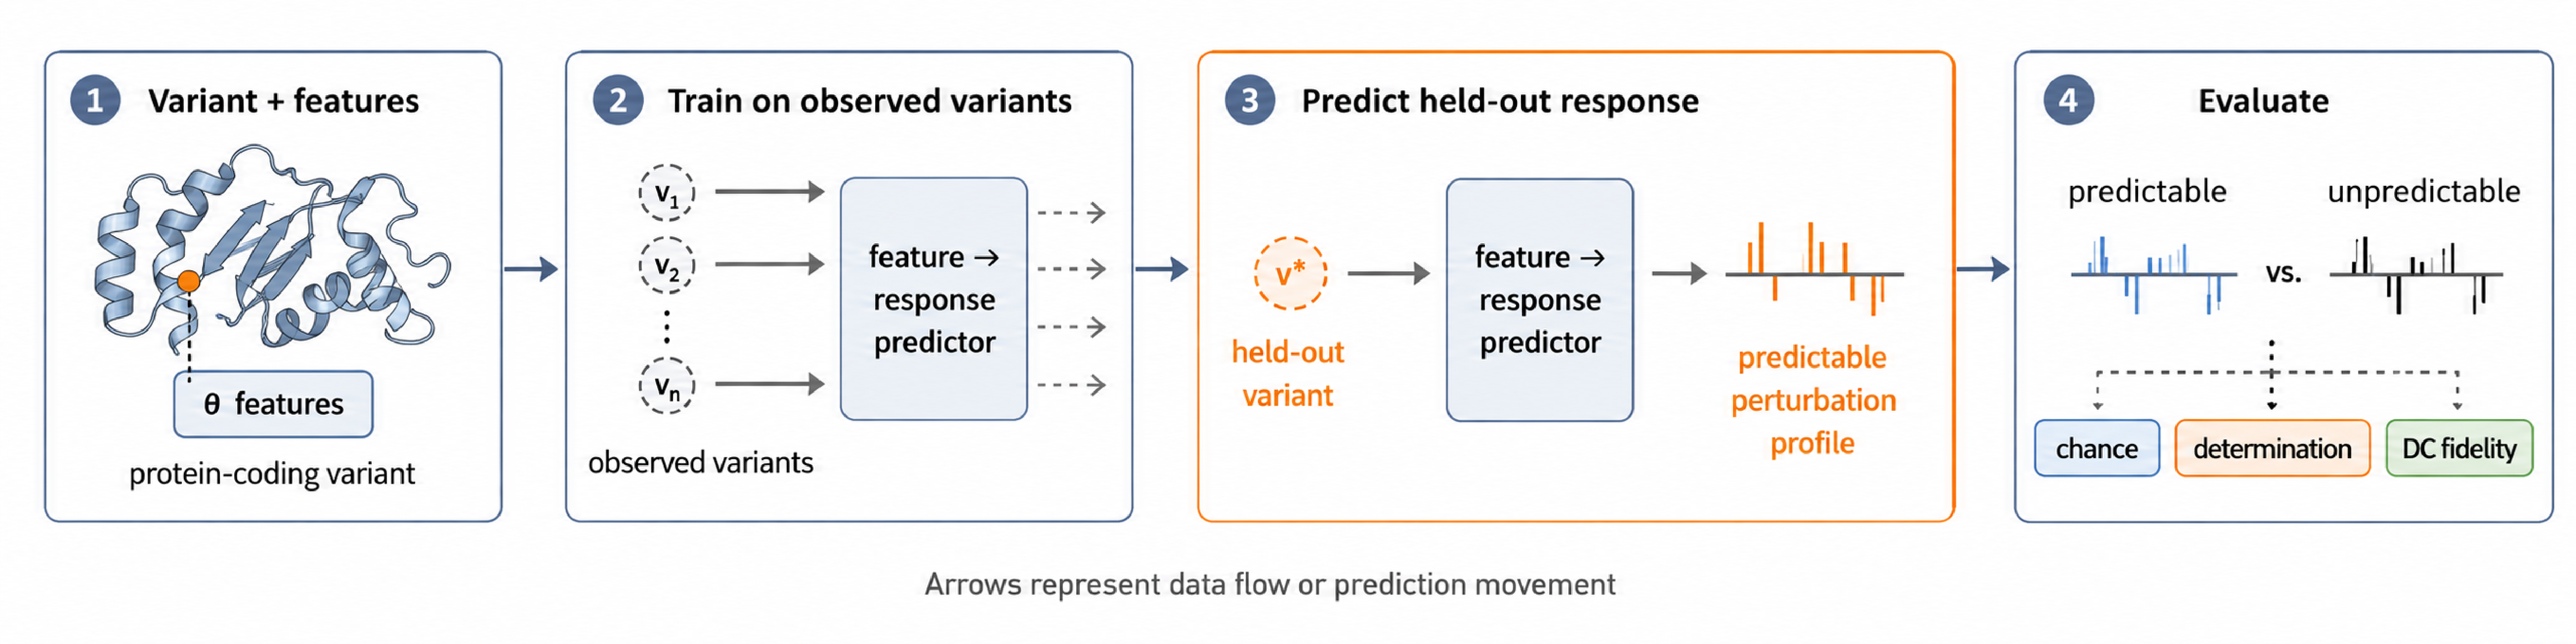
\includegraphics[width=112mm]{Fig1g.pdf}};

  % ---------- panel letters ----------------------------------------------------
  \tikzset{plab/.style={font=\bfseries\large,anchor=north west,inner sep=0}}
  \node[plab] at (1,201.5) {a};
  \node[plab] at (69,201.5) {b};
  \node[plab] at (1,109.5) {c};
  \node[plab] at (57,109.5) {d};
  \node[plab] at (126,109.5) {e};
  \node[plab] at (1,67.5) {f};
  \node[plab] at (66,67.5) {g};
\end{tikzpicture}
\end{document}
